%!TEX root =/Users/ludovicl/Dropbox/Cours/UTBM/P15/RapportStage/main.tex
\chapter{Mise en situation et description des activités du stagiaire}
Lors des discutions avec les fondateurs pendant l'entretien d'embauche je savais que j'allais travaillé sur les technologies Ruby et Python. Le sujet était donc de travailler avec le CTO sur la base de données et de coder le back-end de l'importation de données billetteries.
\\ 

À mon arrivée l'architecture d'une base de données était déjà réalisée. Mais elle n'était pas utilisée et encore moins remplie. J'ai donc du rapidement l'adapter en fonction des premières données billetteries que j'ai reçu et que je devais insérer. Plusieurs stagiaires étaient passés sur la base de données auparavant, certaines tables étaient redondantes (parfois en français et en anglais), certaines autres ne contenaient pas de clés étrangères (juste l'id d'une autre table). J'ai donc au fur et à mesure corrigé tout ça. 


\section{Importation manuel de données billetteries des clients dans ArenaPricing}

L'une de mes premières taches en arrivant dans l'entreprise est de créer un logiciel permettant à Tech4Team et à certains clients de facilement insérer dans notre base de données un fichier CSV\footnote{Comma-separated values, connu sous le sigle CSV, est un format informatique ouvert représentant des données tabulaires sous forme de valeurs séparées par des virgules.} contenant des données billetteries. À terme le but est d'intégrer le logiciel les API des logiciels de billetterie des clients.

\subsection{Le besoin}

Le besoin peut donc être visualisé par le schéma \ref{interface_upload} page \pageref{interface_upload}. Tech4Team ou un client veut insérer des nouveaux tickets dans la base de données Arenapricing. Il sélectionne alors un fichier CSV à la main depuis l'interface web, le site analyse le fichier, extrait les informations importantes et les inserts en base de donnes. Toute la partie d'analyse et d'insertion doit être invisible du point de vue de l'utilisateur.
\\ \\
Le logiciel d'upload doit également être capable de s'interfacer avec des API.

\begin{center}

\includegraphics[scale=0.57]{images/datafit.png}
\captionof{figure}{Principe de l'interface d'upload}
\label{interface_upload}
\end{center}


\subsection{Première réalisation du front d'importation}

Pour réaliser ce site web d'importation nous avons décidé après discussion avec le lead developper d'utiliser le langage Python. Ce langage permet de développer rapidement est dispose d'énormément de modules s'ajoutant aux fonctions de base. Il est ainsi aisé de parser un fichier CSV. J'ai également utilisé le microframework Flask pour créer les pages web en elle même et servir de serveur web. Pour le design du site, j'ai utilisé le framework Zurb Foundation afin d'avoir une identité visuelle cohérente. 

\begin{center}
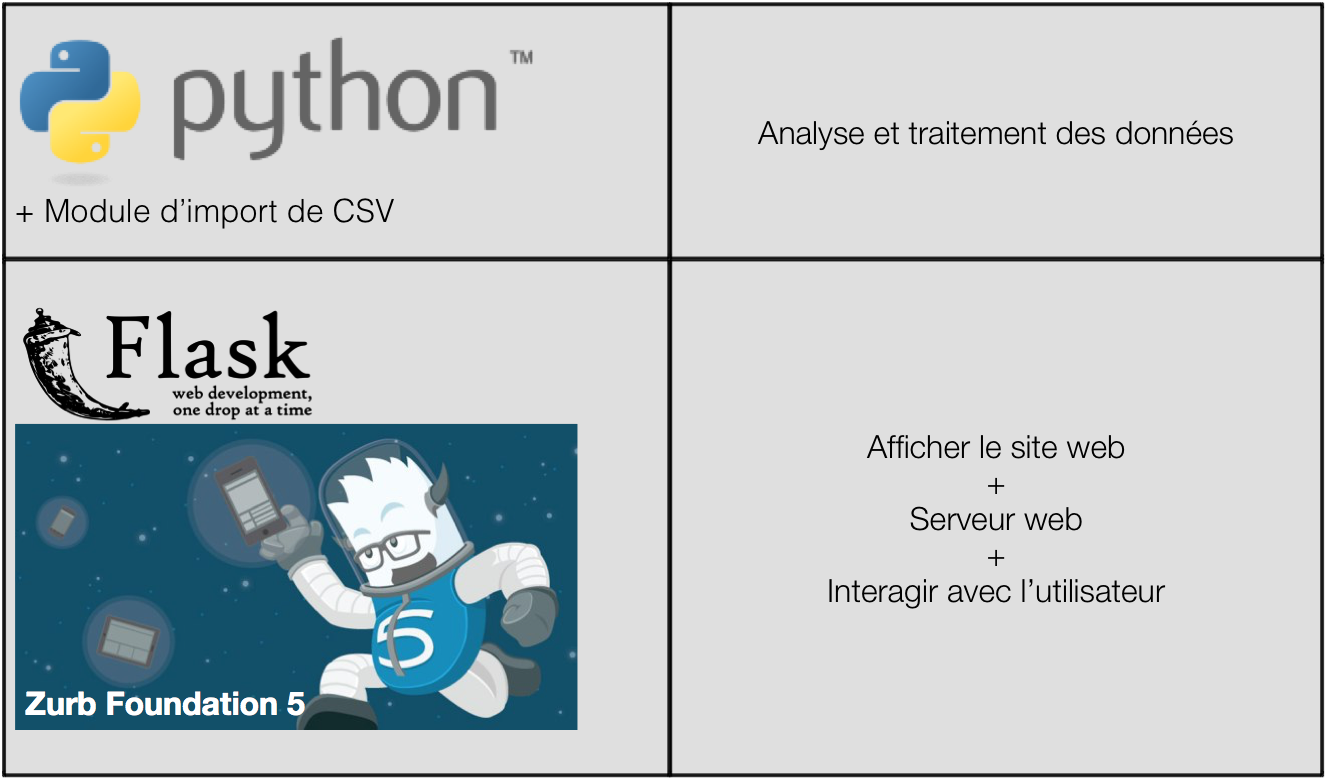
\includegraphics[scale=0.6]{images/datafit2.png}
\captionof{figure}{Téchnologies utilisées pour le front}
\label{interface_upload_tech}
\end{center}

\subsubsection{L'interface homme-machine obtenue}

Comme nous pouvons le voir sur l'impression d'écran \ref{front_upload} page \pageref{front_upload} l'interface est permet à l'utilisateur d'envoyer un fichier CSV préalablement sélectionné.
En plus du nom de l'organisation, nous affichons le type d'événement correspondant au fichier envoyé ainsi que le logiciel de billetterie d'où provient l'export. \\

\begin{center}
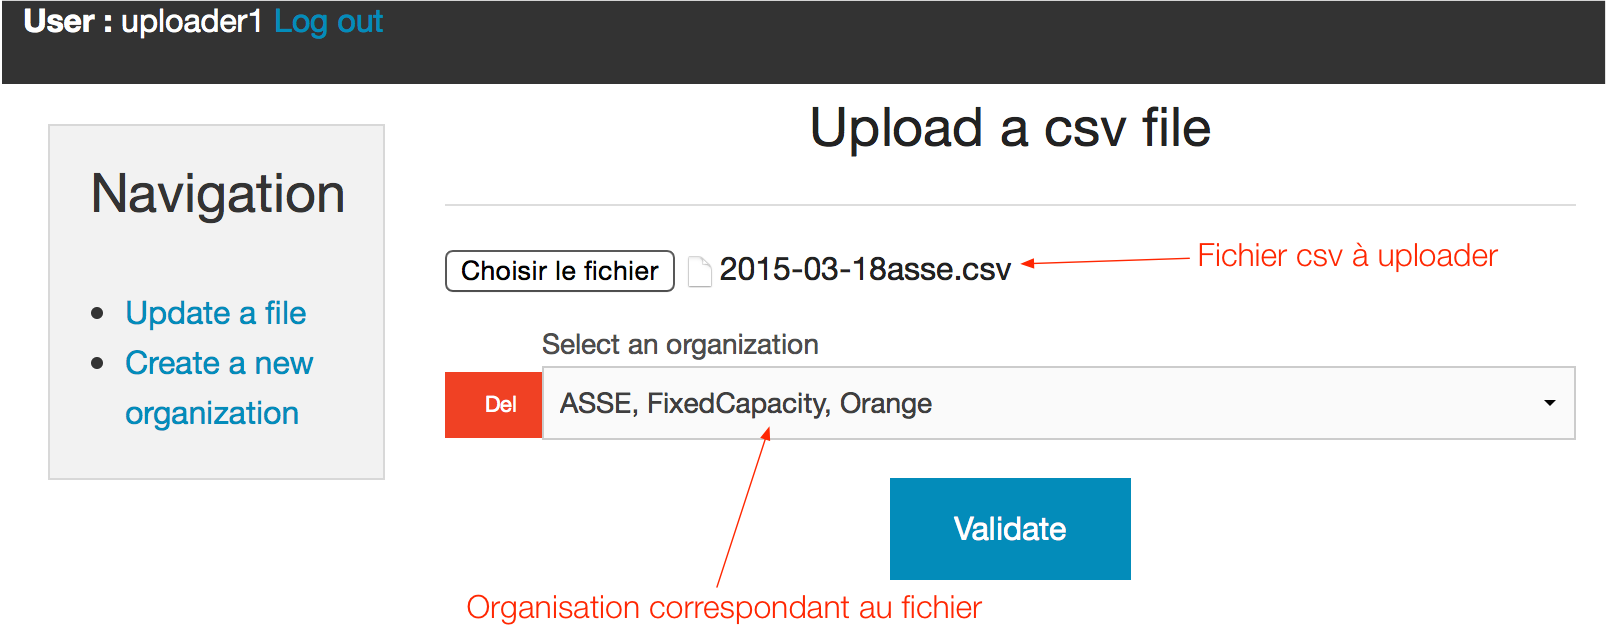
\includegraphics[scale=0.6]{images/front1.png}
\captionof{figure}{Front d'upload d'un fichier CSV}
\label{front_upload}
\end{center}

\subsubsection{Parsing des données en Python}
Pour parser les fichiers CSV j'utilise le module natif CSV.
\\


\lstset{style=custompython}
\begin{lstlisting}
with open(file_path, 'r', encoding=charset['encoding']) as f:

	#read csv file with csv module
	dict_csv = csv.DictReader(f, delimiter=';', quoting=csv.QUOTE_ALL)
	
	#use strategy design pattern with Secutix object
	secutix = ParsingStrategyContext(Secutix())	
	
	#parse dictionay and send organization name, event date, export date
	secutix.parse_file(dict_csv, o_name, e_date, export_date)

#ask object to send data to the ruby. e_type is event type 
reason = secutix.upload_data(e_type)
return reason
\end{lstlisting}
\captionof{lstlisting}{Code analysant le fichier CSV}

\leavevmode \\
La fonction open permet d'ouvrir le fichier $file\_path$, ensuite je récupère le dictionnaire associé à au fichier CSV avec $csv.DictReader$. La méthode $parse\_file$ permet de générer le dictionnaire avec les informations des tickets/achats comme le montre la figure \ref{dict_csv} page \pageref{dict_csv}, nous obtenons finalement une liste de dictionnaire ou chaque entrée de la liste est une ligne du fichier CSV. 

\begin{center}
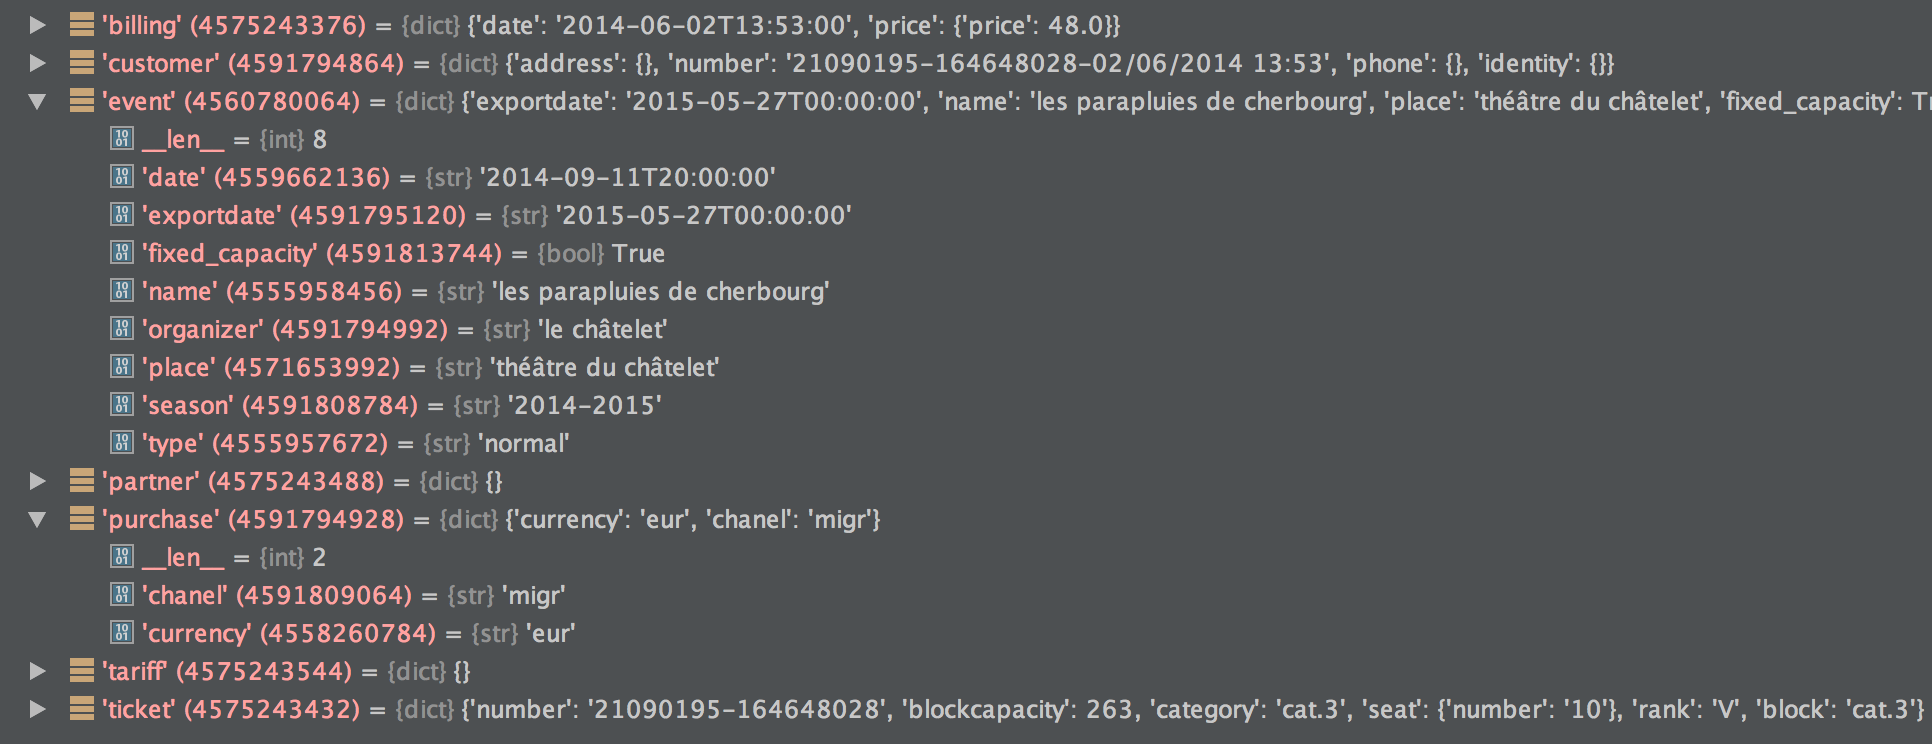
\includegraphics[scale=0.45]{Images/dict_tickets.png}
\captionof{figure}{Dictionnaire récupéré pour une ligne du fichier CSV}
\label{dict_csv}
\end{center}


D'un point de vue architecture de l'application j'utilise le design pattern strategy. Ce design pattern est utile lors qu'un objet peut effectuer plusieurs traitements différents, dépendant d'une variable ou d'un état.

L'implémentation de ce design pattern peut être visualisé sur le diagramme figure \ref{stategy_pattern} page \pageref{dict_csv}.

\begin{center}
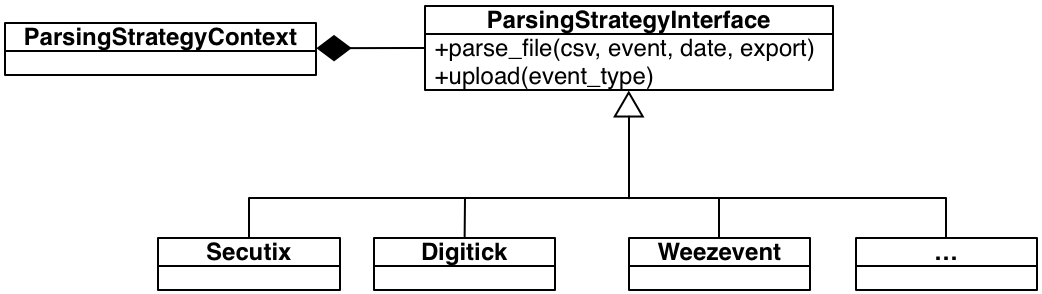
\includegraphics[scale=0.75]{Images/StrategyPattern.png}
\captionof{figure}{Design pattern strategy}
\label{stategy_pattern}
\end{center}



\subsubsection{Problèmatique posée par ce logiciel}
Après avoir testé le logiciel d'importation avec de nombreux clients, il nous apparait que les fichiers fournis ne sont pas génériques. 
Les noms des colonnes ne sont pas les mêmes en fonction des exports alors que le logiciel de billetterie est identique et dans certains cas le changement apparait pour un même client d'une saison à l'autre. 
On se rend donc rapidement compte que nous ne pouvons pas créer un script unique par logiciel de billetterie.
\\ \\
La partie front en Flask n'est acutelelment plus utilisée, mais le python qui permet de parser les données et utilisé pour les clients qui n'ont pas d'API et qui uploadent donc des fichiers CSV sur un serveur FTP. 


\subsection{Deuxième itération pour le logiciel d'import des fichiers}
Nous décidons de repenser notre logiciel pour que le client désirant envoyer un fichier CSV puisse spécifier sur l'interface les champs qu'il souhaite importer.

Comme le montre l'image \ref{draft_front_import2} page \pageref{draft_front_import2} du premier draft que j'ai réalisé, le client doit maintenant faire un travail d'association entre les champs présents dans le fichier CSV leur correspondance réel. 

\begin{center}
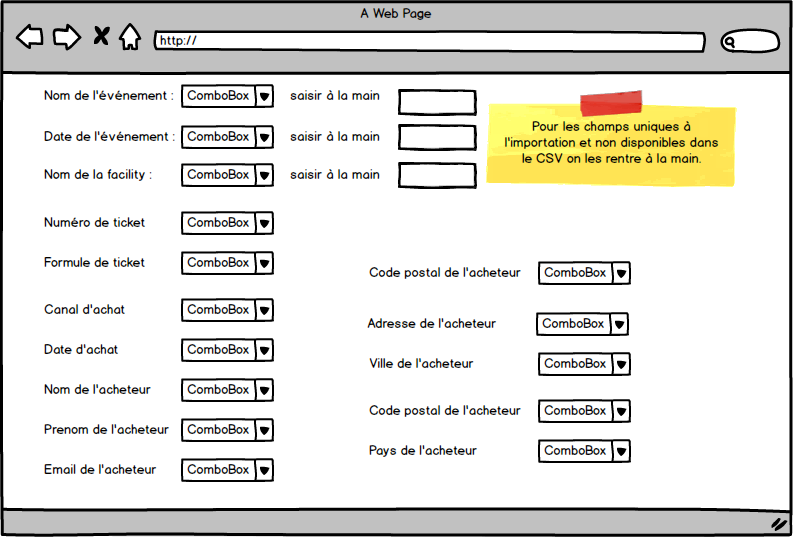
\includegraphics[scale=0.55]{images/front3.png}
\captionof{figure}{Premier draft du logiciel d'importation 2.0}
\label{draft_front_import2}
\end{center}


\subsubsection{Création de l'IHM}
Pour réaliser l'interface d'upload j'ai utilisé le framework Ruby on rails afin pouvoir intégrer facilement la page d'upload au reste du site.

\begin{center}
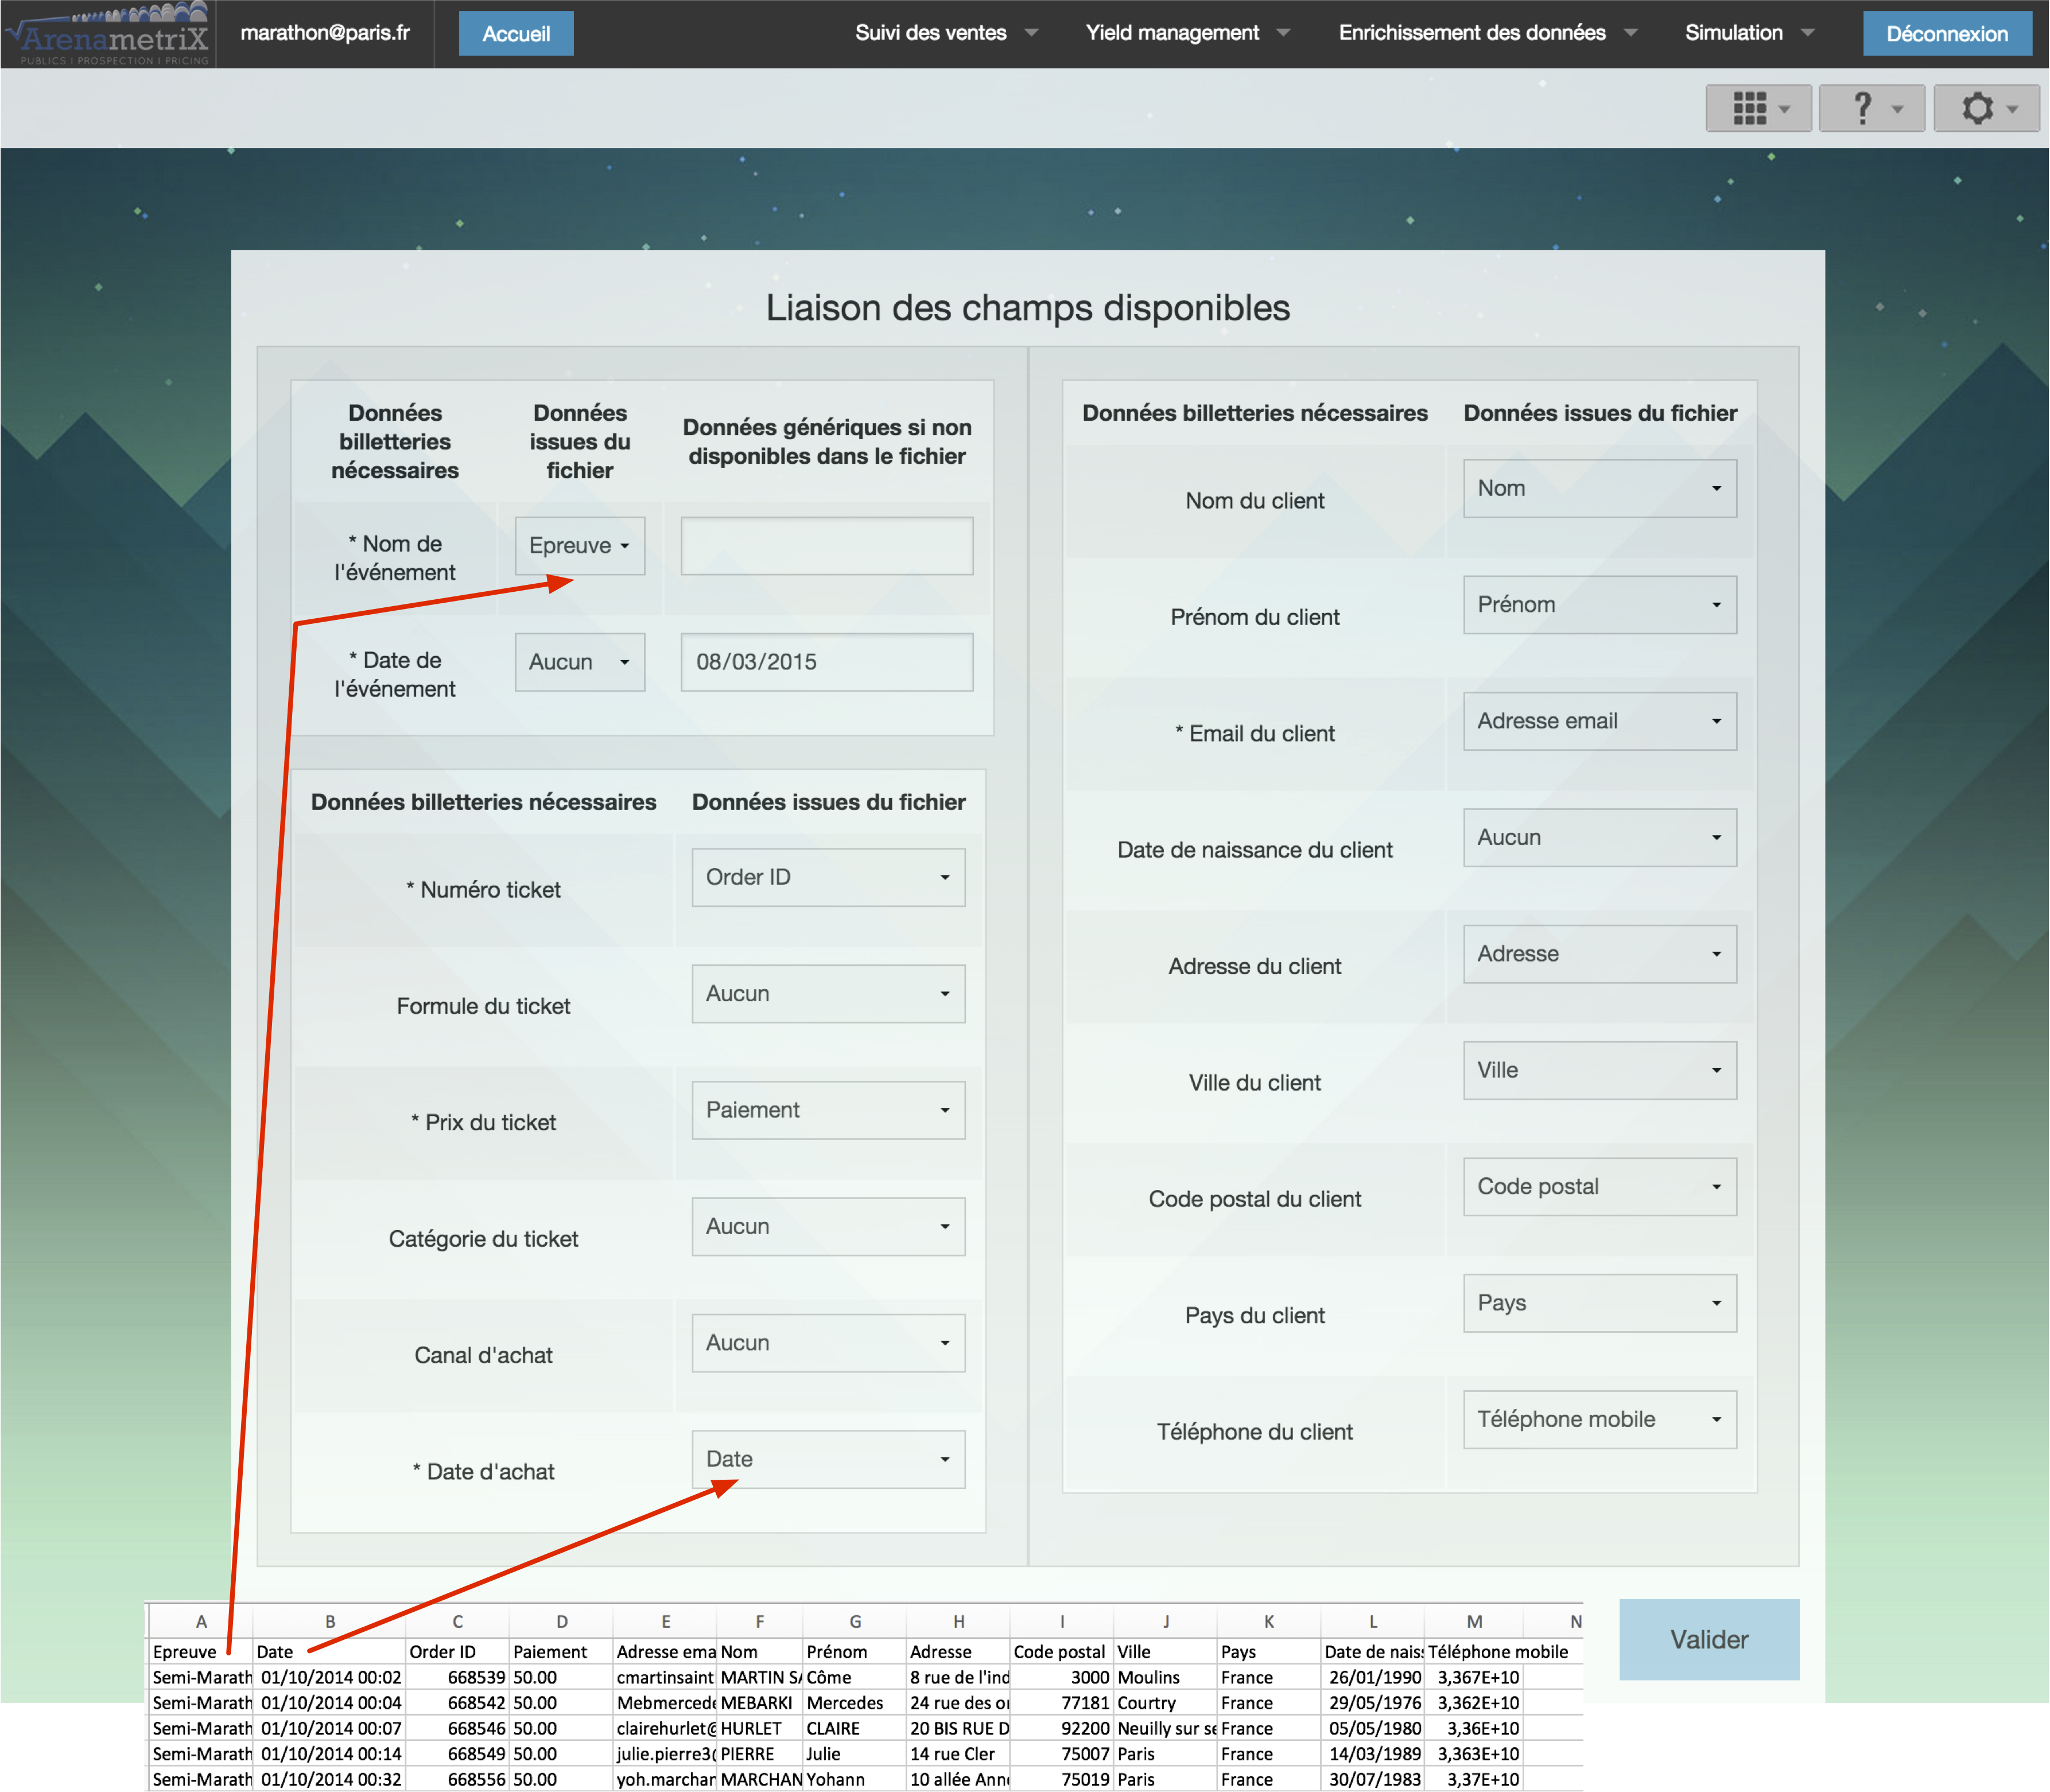
\includegraphics[scale=0.37]{images/final_front2.png}
\captionof{figure}{Logiciel d'importation des clients}
\label{final_front_import2}
\end{center}

J'obtient finalement le front-end \ref{final_front_import2} page \pageref{final_front_import2}, comme nous pouvons le voir avec le fichier CSV de test les champs sont mappés ensemble. Si la donnée n'est pas présente, une insertion vide se fait en base de données. Les champs marqué avec une étoile sont indispensables. Certains champs comme le nom de l'événement et la date peuvent être inscrits à la main s’ils ne sont pas fournis dans le fichier CSV.


\subsubsection{L'importation des fichiers CSV}

Afin d'importer les données dans le logiciel de billéterie j'utilise l'ORM ActiveRecord.

\lstset{style=customruby}
\begin{lstlisting}
begin
  country = Pricing::Country.find_by!(name: customer_country_to_ins)
rescue ActiveRecord::RecordNotFound 
  country = Pricing::Country.new(name: customer_country_to_ins)
end
country.save
begin
  department = Pricing::Department.find_by!(name: customer_zip_to_ins, country: country)
rescue ActiveRecord::RecordNotFound
  department = Pricing::Department.new(name: customer_zip_to_ins,  country: country)
end
department.save
begin
  city = Pricing::City.find_by!(name: customer_city_to_ins, department: department)
rescue ActiveRecord::RecordNotFound
  city = Pricing::City.new(name: customer_city_to_ins,  department: department)
end
city.save
\end{lstlisting}
\captionof{lstlisting}{Exemple de code insérant une adresse}
\leavevmode \

Avant d'insérer une donnée, je vérifie si elle est présente, si ce n'est pas le cas je rescue l'exception et j'insère la donnée. 
L'ORM ActiveRecord permet de s'astreindre des contraintes habituelles du SQL, lorsque je fais coutry: country lors d'une intention de département l'ORM comprend qu'il doit lier country comme clé étrangère de département.

La majorité des clients nous fournissent des fichiers CSV. Ces fichiers sont extraits à partir du logiciel de billetterie utilisé par le client.


\subsection{Les API des logiciels billetteries}
Différentes approches pour importer les données sont possibles : 
\begin{itemize}
  \item[\textbullet] Le client nous donne le login et mot de passe de son logiciel billetterie : nous faisons l'extraction d'un fichier CSV et nous l'importons à la main dans la base de données. 
  \item[\textbullet] Le client envoie son fichier CSV par mail : nous l'importons à la main dans la base de données.
  \item[\textbullet] Le client dépose son fichier CSV sur un serveur FTP : un script python est chargé de régulièrement scanner ce serveur FTP est importer les données si il a un changement.
  \item[\textbullet] La société logiciel billetterie nous donne une clé d'API, ainsi avec le mot de passe et login du client nous pouvons accéder au données en nous connectant directement à la base de données. C'est l'idéal pour nous, cela nous permet d'automatiser les imports.
\end{itemize}

Actuellement nous avons accès aux API des billetteries WeezEvent et Njuko. 

Pour récupérer les données des API j'utilise le module request qui permet de faire des requêtes get.

Ainsi la requête suivante me permet de récupérer les événements d'une organisation :

\lstset{style=custompython}
\begin{lstlisting}
json_events = requests.get("https://api.weezevent.com/events",
                            params={'api_key': API_KEY,
                                    'access_token': token,
                                    'include_closed': True}
                          )
event = json_events.json()['events'].pop()
\end{lstlisting}
\captionof{lstlisting}{Récupération des événements sur l'API de weezevent}
\leavevmode \

À la fin de mon stage, nous avions accès a trois API de logiciel de billetteries : 
\begin{itemize}
  \item[\textbullet] WeezEvent pour les événements :
  \begin{itemize}
	\item Mondial du tatouage : un salon annuel pour les tatoueurs du monde entier
	\item File7 : Une salle de concert en région parisienne. 
	\item Rhum Fest : Un événement et une exposition sur le thème de rhum
  \end{itemize}
  \item[\textbullet] Njuko pour les événements :
  \begin{itemize}
  	\item Marathon de Paris
  \end{itemize}

\end{itemize}

\subsection{La base de données en elle même}
L'architecture de la base de données ArenaPricing peut être visualisée sur la figure \ref{arenapublic-1} de l'annexe page \pageref{arenapublic-1}.



		